\documentclass[11pt,a4paper]{article}

\usepackage[utf8]{inputenc}
\usepackage[T1]{fontenc}
\usepackage{lmodern}
\usepackage[margin=2.5cm]{geometry}
\usepackage{amsmath,amssymb,amsthm}
\usepackage{booktabs}
\usepackage{graphicx}
\usepackage[colorlinks=true,linkcolor=blue,citecolor=blue,urlcolor=blue]{hyperref}

\graphicspath{{../figures/}}
\setlength{\emergencystretch}{2em}

\theoremstyle{plain}
\newtheorem{theorem}{Theorem}
\newtheorem{corollary}[theorem]{Corollary}

% framed box for the two structural ideas of the proof
\newsavebox{\keyboxcontent}
\newenvironment{keyidea}
  {\par\medskip\noindent\begin{lrbox}{\keyboxcontent}%
   \begin{minipage}{\dimexpr\linewidth-2\fboxsep-2\fboxrule\relax}\textbf{Key idea.}\ }
  {\end{minipage}\end{lrbox}\fbox{\usebox{\keyboxcontent}}\par\medskip}

\newcommand{\ket}[1]{\lvert #1\rangle}
\newcommand{\bra}[1]{\langle #1\rvert}
\newcommand{\ketbra}[2]{\lvert #1\rangle\langle #2\rvert}
\newcommand{\C}{\mathbb{C}}
\newcommand{\cC}{\mathcal{C}}
\newcommand{\cW}{\mathcal{W}}
\newcommand{\cH}{\mathcal{H}}
\newcommand{\cR}{\mathcal{R}}
\newcommand{\wt}[1]{\lvert #1\rvert}
\newcommand{\one}{\mathbf{1}}
\DeclareMathOperator{\Tr}{Tr}

\title{Mismatched Petz recovery for the Leung code\\ under weak amplitude damping}
\author{Pierre Levilion}
\date{\today}

\begin{document}

\maketitle

\begin{abstract}
The Petz recovery map is built from a model of the noise. What happens when this model is wrong? We study the four-qubit Leung code under amplitude damping with parameter $\gamma$, recovered by the Petz map built for an assumed parameter $h$. Numerically, the best choice is not $h=\gamma$ but a smaller value, which approaches $\gamma/2$ at weak noise. We prove that for $h=r\gamma$ with $r>0$ fixed,
\[
F(\gamma,r\gamma)=1-\Big[\tfrac74-\Big(1-\tfrac1{\sqrt2}\Big)\,r(1-r)\Big]\gamma^2+O(\gamma^3),
\]
so $r=\frac12$ is optimal, and any underestimate of the noise ($0<r<1$) beats the matched map. 
%The proof rests on two structural facts. First, $236$ of the $256$ traces entering the fidelity vanish identically. Second, the first-order terms cancel, because every Petz map with $h>0$ corrects single decays exactly at leading order.%
\end{abstract}

%======================================================================
\section{Introduction}
%======================================================================

The Petz map is a universal recovery channel. Given a noise channel and a reference state, it provides an explicit decoder whose fidelity is provably close to the optimal one~\cite{barnum2002}. For the Leung code under amplitude damping, our SDP computations show that it is in fact much closer than this bound guarantees: $1-F_{\mathrm{Petz}}\approx1.75\gamma^2$, against $1-F_{\mathrm{opt}}\approx1.25\gamma^2$ for the optimal recovery~\cite{fletcher2007}. Its weak point is that it needs the noise channel itself. In practice a damping rate is estimated, not known, so the decoder is built for an assumed parameter $h$ while the true parameter is $\gamma$. How much fidelity does a wrong guess cost?

We study this question for the four-qubit code of Leung, Nielsen, Chuang and Yamamoto~\cite{leung1997} under independent amplitude damping. Figure~\ref{fig:numerics}(a) shows the gain of the mismatched Petz map over the matched one ($h=\gamma$). It contains two surprises:
\begin{itemize}
  \item \emph{Underestimating the noise helps.} The gain is positive below the diagonal $h=\gamma$ and negative above it. The best assumed value $h^*(\gamma)$ satisfies $h^*/\gamma\approx0.50$ at $\gamma=10^{-3}$, and the ratio decreases to $0.26$ at $\gamma=0.3$ (Figure~\ref{fig:numerics}(b)).
  \item \emph{Assuming no noise at all is catastrophic.} Every $h>0$, however small, gives $1-F=O(\gamma^2)$, whereas at $h=0$ the Petz map reduces to the baseline recovery, with $1-F\approx\frac32\gamma$ (see the notebooks \texttt{petz\_\allowbreak vs\_\allowbreak baseline.ipynb} and \texttt{robustness.ipynb}).
\end{itemize}
This note explains both observations analytically in the weak-noise regime.

\begin{figure}[t]
\centering
\begin{minipage}[b]{0.53\textwidth}
\centering
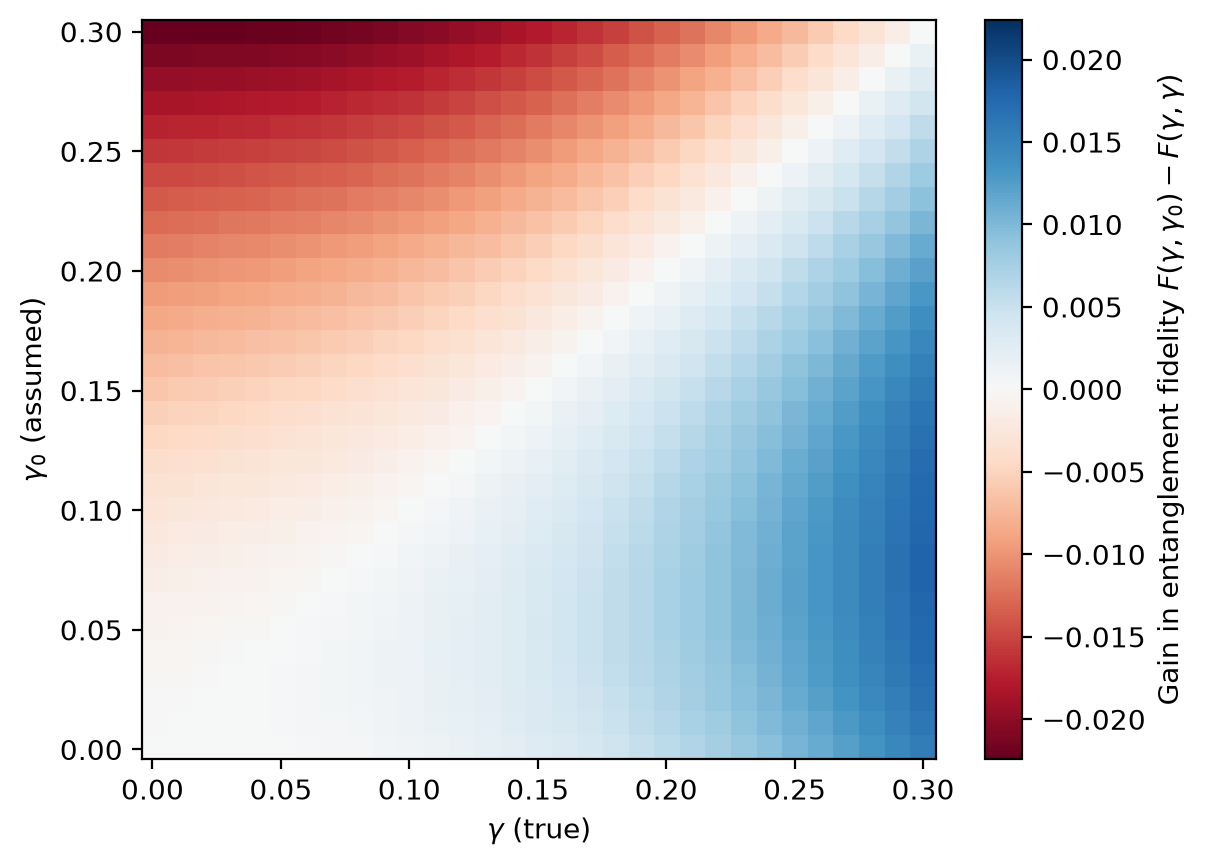
\includegraphics[width=\linewidth]{fidelity_gain_heatmap.png}\\[2pt]
\small (a) gain $F(\gamma,h)-F(\gamma,\gamma)$
\end{minipage}\hfill
\begin{minipage}[b]{0.45\textwidth}
\centering
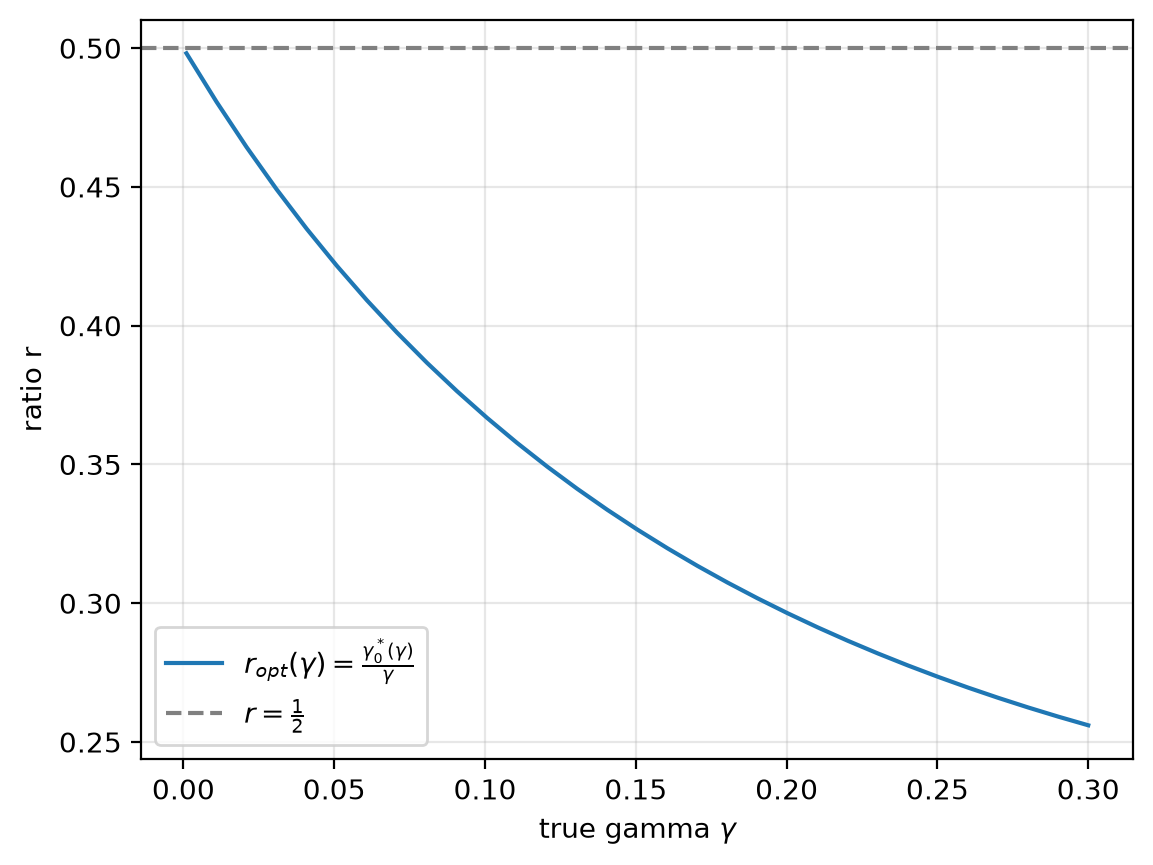
\includegraphics[width=\linewidth]{optimal_calibration_ratio.png}\\[2pt]
\small (b) optimal ratio $h^*(\gamma)/\gamma$
\end{minipage}
\caption{Numerics from the notebooks \texttt{robustness.ipynb} and \texttt{petz\_calibration.ipynb}; the assumed parameter $h$ is written $\gamma_0$ on the axes. (a)~Gain of the Petz map built for $h$ over the matched map; blue means that the miscalibrated map is better. (b)~The assumed parameter $h^*(\gamma)$ that maximises $F(\gamma,h)$, divided by $\gamma$. The dashed line is the weak-noise limit $\frac12$ predicted by Theorem~\ref{thm:main}.}
\label{fig:numerics}
\end{figure}

%======================================================================
\section{Mathematical setting}
%======================================================================

\paragraph{Noise.} Amplitude damping with parameter $\gamma\in[0,1]$ has Kraus operators $K_0(\gamma)=\ketbra00+\sqrt{1-\gamma}\,\ketbra11$ and $K_1(\gamma)=\sqrt\gamma\,\ketbra01$. On four qubits the Kraus operators are $N_j(\gamma)=K_{j_1}(\gamma)\otimes\cdots\otimes K_{j_4}(\gamma)$, labelled by bit strings $j=j_1j_2j_3j_4$, where $j_i=1$ means that qubit $i$ decayed. We write $\wt{j}$ for the number of decays and $\bar j$ for the complementary string.

\paragraph{Code.} The Leung code is spanned by $\ket{0_L}=\frac1{\sqrt2}(\ket{0000}+\ket{1111})$ and $\ket{1_L}=\frac1{\sqrt2}(\ket{0011}+\ket{1100})$. Its encoding isometry is $V=\ketbra{0_L}0+\ketbra{1_L}1$ and its code projector is $\Pi=VV^\dagger$. The code is supported on $\cC=\cC_0\cup\cC_1$, where $\cC_0=\{0000,1111\}$ and $\cC_1=\{0011,1100\}$. The encoded noise channel $\Phi_\gamma$ has the $16$ Kraus operators $E_j(\gamma)=N_j(\gamma)V\in\C^{16\times2}$.

\paragraph{Mismatched Petz map.} The Petz map built for the assumed parameter $h$, with reference state $I_2/2$, has the Kraus operators
\begin{equation}\label{eq:petz}
R_k(h)=\frac1{\sqrt2}\,E_k(h)^\dagger\,\tau_h^{-1/2},\qquad \tau_h=\Phi_h\Big(\frac{I_2}2\Big)=\frac12\sum_jE_j(h)E_j(h)^\dagger .
\end{equation}
For $0<h<1$, $\tau_h$ is invertible (Section~\ref{sec:proof}). Hence $\sum_kR_k^\dagger R_k=\tau_h^{-1/2}\tau_h\tau_h^{-1/2}=I_{16}$, and the map is trace preserving without any completion. At $h=0$, by contrast, $\tau_0=\Pi/2$ is singular. With a pseudo-inverse and a completion on $\ker\tau_0$, as in the code, the map becomes the baseline recovery $\cR_0(X)=V^\dagger XV+\Tr[(I-\Pi)X]\,I_2/2$.

\paragraph{Fidelity.} The entanglement fidelity of a qubit channel with Kraus operators $L_i$ is $\frac14\sum_i|\Tr L_i|^2$. The composition $\cR_h\circ\Phi_\gamma$ has the $256$ Kraus operators $R_k(h)E_j(\gamma)$, so
\begin{equation}\label{eq:F}
F(\gamma,h)=\frac18\sum_{k,j}T_{kj}^2,\qquad T_{kj}(\gamma,h)=\Tr\Big(E_k(h)^\dagger\,\tau_h^{-1/2}\,E_j(\gamma)\Big)\in\mathbb R .
\end{equation}

%======================================================================
\section{Main result}
%======================================================================

\begin{theorem}\label{thm:main}
Fix $r>0$ and set $h=r\gamma$. As $\gamma\to0^+$,
\begin{equation}\label{eq:main}
\boxed{\;F(\gamma,r\gamma)=1-c(r)\,\gamma^2+O(\gamma^3),\qquad c(r)=\frac74+(1-\frac1{\sqrt2})\,r(r-1).\;}
\end{equation}
\end{theorem}

Since $r(1-r)=\frac14-(r-\frac12)^2$, the coefficient can also be written $c(r)=\frac32+\frac{\sqrt2}8+(1-\frac1{\sqrt2})\,(r-\frac12)^2$. This form gives the consequences for calibration.

\begin{corollary}\label{cor:calibration}
Let $c$ be as in \eqref{eq:main}.
\begin{enumerate}
  \item[(a)] \emph{Matched map:} $1-F(\gamma,\gamma)=\frac74\gamma^2+O(\gamma^3)$.
  \item[(b)] \emph{Best calibration:} $c$ is minimal at $r=\frac12$, so the best Petz map is built for half the true noise, with $c(\frac12)=\frac32+\frac{\sqrt2}8\approx1.677$. Its gain over the matched map is $F(\gamma,\frac\gamma2)-F(\gamma,\gamma)=\frac{2-\sqrt2}8\gamma^2+O(\gamma^3)\approx0.073\,\gamma^2$.
  \item[(c)] \emph{Sign of the error:} $c(r)<c(1)$ if and only if $0<r<1$. At leading order, any underestimate of the noise helps and any overestimate hurts, which is the sign pattern of Figure~\ref{fig:numerics}(a).
  \item[(d)] \emph{Optimal ratio:} if $0<r_1<\frac12<r_2$, every maximiser $r^*(\gamma)$ of $r\mapsto F(\gamma,r\gamma)$ on $[r_1,r_2]$ satisfies $|r^*(\gamma)-\frac12|=O(\sqrt\gamma)$.
\end{enumerate}
\end{corollary}

\begin{proof}
Parts (a)--(c) follow from the two forms of $c$. For (d), let $f_\gamma(r)=(1-F(\gamma,r\gamma))/\gamma^2$. The uniform remainder gives $|f_\gamma(r)-c(r)|\le C\gamma$ on $[r_1,r_2]$. Since $r^*$ minimises $f_\gamma$, we get $(1-\frac1{\sqrt2})(r^*-\frac12)^2=c(r^*)-c(\frac12)\le f_\gamma(r^*)-f_\gamma(\frac12)+2C\gamma\le2C\gamma$.
\end{proof}

Note also that $\lim_{r\to0^+}c(r)=c(1)=\frac74$. At this order, a Petz map built for a vanishingly small but non-zero noise is exactly as good as the matched one.

%======================================================================
\section{Proof outline}\label{sec:proof}
%======================================================================

The proof is a direct computation, organised so that most of the $256$ traces in \eqref{eq:F} never need to be computed. The detailed matrices are collected in the appendix. All formulas below were checked symbolically and against the numerical code.

\subsection*{Step 1: each Kraus column is a single basis vector, except for no decay}

A decay pattern $j$ acts on a basis state by turning the decayed $1$'s into $0$'s:
\[
N_j(\gamma)\ket x=\gamma^{\wt{j}/2}(1-\gamma)^{(\wt{x}-\wt{j})/2}\ket{x-j}\quad\text{if } j\preceq x,\qquad N_j(\gamma)\ket x=0\quad\text{otherwise},
\]
where $j\preceq x$ means that $x$ has a $1$ wherever $j$ does. Applied to the codewords, this gives the two columns of $E_j$:
\begin{align}
\sqrt2\,E_j(\gamma)\ket0&=\delta_{j,0000}\ket{0000}+\gamma^{\wt{j}/2}(1-\gamma)^{(4-\wt{j})/2}\ket{\bar j},\label{eq:col0}\\
\sqrt2\,E_j(\gamma)\ket1&=\gamma^{\wt{j}/2}(1-\gamma)^{(2-\wt{j})/2}\big(\one[j\preceq0011]\ket{0011-j}+\one[j\preceq1100]\ket{1100-j}\big).\label{eq:col1}
\end{align}
Table~\ref{tab:columns} in the appendix lists all $32$ columns. Two features matter:
\begin{itemize}
  \item Every column is a multiple of a \emph{single} basis vector, except the two columns of the no-decay operator $E_{0000}$, which lie in $\operatorname{span}\cC_0$ and $\operatorname{span}\cC_1$.
  \item A single decay ($\wt{j}=1$) sends $\ket{0_L}$ to $\ket{\bar j}$, of weight $3$, and $\ket{1_L}$ to $\ket{j'}$, the other weight-one string of the same pair $\{0001,0010\}$ or $\{0100,1000\}$. The four single decays therefore leave eight distinct, mutually orthogonal syndromes.
\end{itemize}

\subsection*{Step 2: \texorpdfstring{$\tau_h$}{tau\_h} is block diagonal}

By \eqref{eq:petz}, $\bra x\tau_h\ket y=\frac12\sum_j\big(N_j(h)^\dagger\ket x\big)^\dagger\,\Pi\,\big(N_j(h)^\dagger\ket y\big)$, and $N_j^\dagger\ket x\propto\ket{x+j}$ re-excites the decayed qubits. This vector is zero unless $x$ has a $0$ wherever $j$ has a $1$. Then each term in the sum is proportional to $\bra{x+j} \Pi \ket{x+y}$ which is non zero when both strings are in the same $\cC_l$. For $x\ne y$ this forces $x+j$ and $y+j$ to be complementary. That is only possible if $j=0000$ and $y=\bar x$ with $\{x,\bar x\}=\cC_0$ or $\cC_1$. Hence, after reordering the basis,
\begin{equation}\label{eq:blocks}
\tau_h\cong B_0(h)\oplus B_1(h)\oplus\lambda_3(h)I_4\oplus\lambda_1(h)I_4\oplus\lambda_2(h)I_4 .
\end{equation}
Here $B_0$ acts on $\cH_0=\operatorname{span}\{\ket{0000},\ket{1111}\}$, $B_1$ acts on $\cH_1=\operatorname{span}\{\ket{0011},\ket{1100}\}$, and the twelve remaining basis states are eigenvectors:
\[
B_0=\frac14\begin{pmatrix}(1+h^2)^2&(1-h)^2\\(1-h)^2&(1-h)^4\end{pmatrix},\qquad
B_1=\frac{(1-h)^2}4\begin{pmatrix}1+h^2&1\\1&1+h^2\end{pmatrix},
\]
\[
\lambda_1=\tfrac14h(1-h)(1+h^2)\ \ (\wt{x}=1),\qquad \lambda_2=\tfrac14h^2(1-h)^2\ \ (x\in\cW),\qquad \lambda_3=\tfrac14h(1-h)^3\ \ (\wt{x}=3),
\]
where $\cW=\{0101,0110,1001,1010\}$ are the four weight-two strings outside $\cC$. All blocks are positive definite for $0<h<1$, so $\tau_h$ is invertible. The inverse square root $\tau_h^{-1/2}$ has the same block structure, with explicit blocks given in Appendix~\ref{app:tau}.

\subsection*{Step 3: why only 20 of the 256 traces survive}

Write $\tilde e_{j,\ell}=\sqrt2\,E_j\ket\ell$ for the columns. Then,
\begin{equation}\label{eq:trace}
T_{kj}=\frac12\sum_{\ell\in\{0,1\}}\tilde e_{k,\ell}(h)^T\,\tau_h^{-1/2}\,\tilde e_{j,\ell}(\gamma).
\end{equation}
Two facts now decide which traces can be non-zero:
\begin{enumerate}
  \item the trace only pairs \emph{the same} column $\ell$ of $E_k(h)$ and $E_j(\gamma)$;
  \item by \eqref{eq:blocks}, $\tau_h^{-1/2}$ maps each of the $14$ orthogonal subspaces $\cH_0$, $\cH_1$ and $\C\ket x$ ($x\notin\cC$) into themselves.
\end{enumerate}
So $T_{kj}\ne0$ requires some $\ell$ for which column $\ell$ of $E_k$ and column $\ell$ of $E_j$ lie in the same subspace. By Step~1, every non-zero column lies in exactly one subspace, as listed in Table~\ref{tab:blocks}.

\begin{table}[ht]
\centering
\renewcommand{\arraystretch}{1.25}
\begin{tabular}{@{}lll@{}}
\toprule
block & column $\ell=0$ of $E_j$ for & column $\ell=1$ of $E_j$ for\\
\midrule
$\cH_0$ & $j=0000,\ 1111$ & $j=0011,\ 1100$\\
$\cH_1$ & $j=0011,\ 1100$ & $j=0000$\\
$\C\ket x$, $\wt{x}=3$ & $j=\bar x$ & ---\\
$\C\ket x$, $\wt{x}=1$ & $j=\bar x$ & $j=x'$\\
$\C\ket x$, $x\in\cW$ & $j=\bar x$ & ---\\
\bottomrule
\end{tabular}
\caption{Which columns land in which block of $\tau_h^{-1/2}$. The column $\ell=1$ vanishes for $j\in\cW$, $\wt{j}=3$ and $j=1111$.}
\label{tab:blocks}
\end{table}

Reading the table :
\begin{itemize}
  \item a block $\C\ket x$ receives at most one column for each $\ell$, so it only produces diagonal traces $T_{jj}$; this gives the $3\times 4=12$ traces with $j\notin\cC$;
  \item $\cH_0$ with $\ell=0$ couples $0000$ and $1111$, which gives $4$ traces;
  \item $\cH_1$ with $\ell=0$ and $\cH_0$ with $\ell=1$ couple $0011$ and $1100$, which gives $4$ traces;
  \item a mixed pair such as $(0000,0011)$ never meets: for $\ell=0$ its columns lie in $\cH_0$ and $\cH_1$, and for $\ell=1$ in $\cH_1$ and $\cH_0$.
\end{itemize}
In total $12+4+4=20$ traces survive, and the other $236$ vanish identically.


\subsection*{Step 4: the twenty traces, and why single decays are corrected for every \texorpdfstring{$h>0$}{h > 0}}

Each surviving trace is a product of a few coefficients from \eqref{eq:col0}--\eqref{eq:col1} with one entry of $\tau_h^{-1/2}$. For a single decay ($\wt{j}=1$) the two columns lie in the blocks $\C\ket{\bar j}$ and $\C\ket{j'}$, where $\tau_h^{-1/2}$ is multiplication by $\lambda_3(h)^{-1/2}$ and by $\lambda_1(h)^{-1/2}$. This gives:
\begin{equation}\label{eq:cancel}
\text{for $\ell = 0$ : }\tfrac12\,h^{1/2}(1-h)^{3/2}\,\lambda_3(h)^{-1/2}=1,\qquad \text{ for $\ell = 1$ : } \tfrac12\,\big(h(1-h)\big)^{1/2}\lambda_1(h)^{-1/2}=(1+h^2)^{-1/2}.
\end{equation}
Therefore
\begin{equation}\label{eq:T1}
T_{(1)}:=T_{jj}=\sqrt{\gamma(1-\gamma)}\,\Big[(1-\gamma)+\frac1{\sqrt{1+h^2}}\Big]\qquad(\wt{j}=1).
\end{equation}
At leading order this does not depend on $h$ at all: on the syndromes of a single decay, $R_j(h)$ acts as the ideal correction, whatever $h>0$. The other diagonal traces are $T_{(\cW)}=\gamma(1-\gamma)$ for $j\in\cW$ and $T_{(3)}=h\gamma^{3/2}(1-\gamma)^{1/2}(1+h^2)^{-1/2}$ for $\wt{j}=3$. The no-decay trace involves both $B_0^{-1/2}$ and $B_1^{-1/2}$:
\begin{equation}\label{eq:T00}
T_{0000,0000}=\frac{1+(1-\gamma)^2u}{t}+\frac{2(1-\gamma)}w,
\end{equation}
where $w=\sqrt{2+h^2}$, $u=(1-h)^2+hw$ and $t=\sqrt{1+u^2}$.
The seven remaining traces, in $\cC_0\times\cC_0$ and $\cC_1\times\cC_1$, are listed in Appendix~\ref{app:traces}. At order $\gamma^2$, only the pair $T_{0011,0011}=T_{1100,1100}=\gamma+O(\gamma^2)$ matters. With multiplicities, \eqref{eq:F} becomes
\begin{equation}\label{eq:Fexact}
8F(\gamma,h)=T_{0000,0000}^2+4T_{(1)}^2+4T_{(\cW)}^2+2T_{0011,0011}^2+\rho(\gamma,h),
\end{equation}
where $\rho$ collects the squares of the nine other traces (Appendix~\ref{app:traces}). It is of order $\gamma^4$ when $h=r\gamma$.

\subsection*{Step 5: why the first-order terms cancel}

Put $h=r\gamma$ and expand. From \eqref{eq:T1} and \eqref{eq:T00},
\[
T_{0000,0000}^2=8-16\gamma+O(\gamma^2),\qquad 4T_{(1)}^2=16\gamma+O(\gamma^2),
\]
and all other terms of \eqref{eq:Fexact} are $O(\gamma^2)$. The two first-order terms cancel exactly, for every $r>0$.

\begin{keyidea}
Even when no decay happens, the state loses amplitude: $E_{0000}$ shrinks $\ket{1111}$, $\ket{0011}$ and $\ket{1100}$. So the no-decay branch carries only the fraction $\frac12\Tr E_{0000}^\dagger E_{0000}=1-2\gamma+O(\gamma^2)$ of the total weight, and the missing $2\gamma$ sits in the four single-decay branches. By \eqref{eq:cancel}, the Petz map returns all of it to the code space, for any $h>0$. Nothing is lost at first order, so $r$ can only appear at order $\gamma^2$.
\end{keyidea}

\subsection*{Step 6: where the coefficient \texorpdfstring{$c(r)$}{c(r)} comes from}

At order $\gamma^2$, the $r$-dependence comes only from $T_{0000,0000}$. Up to $O(h^3)$, the quantities in \eqref{eq:T00} expand as
\[
\frac1t=\frac1{\sqrt2}\Big[1+\frac{2-\sqrt2}2\,h+\frac{1-2\sqrt2}4\,h^2\Big],\qquad
\frac ut=\frac1{\sqrt2}\Big[1-\frac{2-\sqrt2}2\,h+\frac{6\sqrt2-7}4\,h^2\Big],
\]
\[
\frac2w=\sqrt2-\frac{\sqrt2}4\,h^2 .
\]
We then split the first term of \eqref{eq:T00} as
\[
\frac{1+(1-\gamma)^2u}t=\Big(\frac1t+\frac ut\Big)-(2\gamma-\gamma^2)\,\frac ut ,
\]
where the terms linear in $h$ cancel inside the bracket. This gives
\begin{equation}\label{eq:T00exp}
T_{0000,0000}=2\sqrt2-2\sqrt2\,\gamma+\Big[\frac{\sqrt2}2+\underbrace{(\sqrt2-1)\,r}_{\text{cross term }\gamma\cdot h}\ \underbrace{-\,(\sqrt2-1)\,r^2}_{\text{terms in }h^2}\Big]\gamma^2+O(\gamma^3).
\end{equation}
The term linear in $r$ is a cross term: it pairs the true deformation $(1-\gamma)^2\approx1-2\gamma$ of the codeword $\ket{0_L}$ with the first-order dependence of the map on $h$, and it rewards building the map for a larger $h$. The term in $r^2$ is a pure $h^2$ effect of the map itself and penalises a large $h$. The two coefficients are equal and opposite. This produces $r(1-r)$, which is maximal at $r=\frac12$ and takes the same value as $r\to0^+$ and at $r=1$. Squaring \eqref{eq:T00exp} and collecting all contributions to \eqref{eq:Fexact} gives Table~\ref{tab:collect}.

\begin{table}[ht]
\centering
\renewcommand{\arraystretch}{1.3}
\begin{tabular}{@{}lccc@{}}
\toprule
contribution & $\gamma^0$ & $\gamma^1$ & $\gamma^2$\\
\midrule
$T_{0000,0000}^2$ & $8$ & $-16$ & $12+(8-4\sqrt2)\,r(1-r)$\\
$4T_{(1)}^2$ & $0$ & $+16$ & $-32$\\
$4T_{(\cW)}^2$ & $0$ & $0$ & $+4$\\
$2T_{0011,0011}^2$ & $0$ & $0$ & $+2$\\
$\rho$ & $0$ & $0$ & $0$\\
\midrule
$8F(\gamma,r\gamma)$ & $8$ & $0$ & $-14+(8-4\sqrt2)\,r(1-r)$\\
\bottomrule
\end{tabular}
\caption{Coefficients of $\gamma^0$, $\gamma^1$ and $\gamma^2$ in \eqref{eq:Fexact} at $h=r\gamma$.}
\label{tab:collect}
\end{table}

Dividing by $8$, and using $\frac{8-4\sqrt2}8=1-\frac1{\sqrt2}=\kappa$, gives Theorem~\ref{thm:main}. As for the remainder: the factors $\sqrt\gamma$ in $T_{(1)}$ and $T_{(3)}$ only enter through their squares, so the right-hand side of \eqref{eq:Fexact} is a smooth function of $(\gamma,r)$ near $\gamma=0$. Taylor's theorem then bounds the remainder by $O(\gamma^3)$, uniformly for $r$ in compact sets.

%======================================================================
\section{Numerical verification and discussion}\label{sec:numerics}
%======================================================================

\paragraph{Leading coefficient.} Table~\ref{tab:check} compares $(1-F(\gamma,r\gamma))/\gamma^2$, computed with the function \texttt{mismatched\_\allowbreak petz\_\allowbreak fidelity}, with $c(r)$. The difference shrinks linearly in $\gamma$, as expected from the $O(\gamma^3)$ remainder. The twenty traces of Step~4 agree with a direct numerical evaluation to about $10^{-15}$, and the other $236$ vanish. Below $\gamma\approx10^{-4}$ the numerical code loses accuracy, because of the eigenvalues of order $h^2$ in $\tau_h$. The closed form \eqref{eq:Fexact}, evaluated in high precision, keeps converging to $c(r)$.

\begin{table}[ht]
\centering
\renewcommand{\arraystretch}{1.2}
\begin{tabular}{@{}lcccc@{}}
\toprule
$r$ & $\gamma=10^{-1}$ & $\gamma=10^{-2}$ & $\gamma=10^{-3}$ & $c(r)$\\
\midrule
$1/4$ & $1.6298$ & $1.6889$ & $1.6945$ & $1.6951$\\
$1/2$ & $1.6311$ & $1.6728$ & $1.6764$ & $1.6768$\\
$1$ & $1.7624$ & $1.7528$ & $1.7503$ & $1.7500$\\
$2$ & $2.5087$ & $2.3580$ & $2.3380$ & $2.3358$\\
\bottomrule
\end{tabular}
\caption{$(1-F(\gamma,r\gamma))/\gamma^2$ from the code, compared with the coefficient $c(r)$ of Theorem~\ref{thm:main}.}
\label{tab:check}
\end{table}

\paragraph{Optimal calibration.} The optimiser \texttt{optimal\_\allowbreak petz\_\allowbreak calibration} gives $h^*/\gamma=0.497$ at $\gamma=10^{-3}$ and $0.482$ at $\gamma=10^{-2}$, approaching $\frac12$ (Figure~\ref{fig:numerics}(b)). At $\gamma=10^{-3}$ the gain over the matched map is $7.39\times10^{-8}$, against $\frac{2-\sqrt2}8\gamma^2=7.32\times10^{-8}$. At larger $\gamma$ higher orders take over: the optimal ratio drops to $0.37$ at $\gamma=0.1$ and $0.26$ at $\gamma=0.3$, and the gain exceeds the $\gamma^2$ prediction ($1.37\times10^{-3}$ against $0.73\times10^{-3}$ at $\gamma=0.1$).

\paragraph{Comparison with optimal recovery.} The SDP-optimal recovery~\cite{fletcher2007} gives $(1-F_{\mathrm{opt}})/\gamma^2\approx1.250$ for $\gamma\le0.05$ (\texttt{data/fidelities.csv}). At weak noise, the best calibration therefore closes only $(c(1)-c(\frac12))/(c(1)-1.25)\approx15\%$ of the gap between the matched Petz map and the optimum. It helps more at stronger noise: at $\gamma=0.3$ it raises $F$ from $0.849$ to $0.867$, against $F_{\mathrm{opt}}=0.890$, which closes $44\%$ of the gap. The constant $1.25$ is a numerical observation, not part of the theorem.

\paragraph{The singular point $h=0$.} Theorem~\ref{thm:main} gives $c(0^+)=\frac74$, yet the map used at $h=0$ is much worse. The formulas of Step~4 are continuous at $h=0$, so
\[
F(\gamma,0^+)=\lim_{h\to0^+}F(\gamma,h)=1-\tfrac74\gamma^2+\tfrac34\gamma^3+\tfrac14\gamma^4 .
\]
For the baseline map $\cR_0$, the trace $\Tr V^\dagger E_j(\gamma)$ is non-zero only for $j=0000$ and $j=1111$, and the completion contributes $\frac18\sum_{j,\ell}\|(I-\Pi)E_j\ket\ell\|^2$. This gives
\[
F(\gamma,0)=1-\tfrac32\gamma+\gamma^2-\tfrac14\gamma^3,\qquad F(\gamma,0^+)-F(\gamma,0)=\tfrac\gamma4(1-\gamma)^2(6+\gamma).
\]
The reason for the jump is the cancellation \eqref{eq:cancel}. For every $h>0$, the single-decay syndromes lie in the support of $\tau_h$, with weight of order $h$, and the Petz map rescales them by $h^{-1/2}$, recovering them fully. At $h=0$ they lie outside the support. The completion then replaces these branches by the maximally mixed state, which keeps only $\frac14$ of their weight $2\gamma$ in the fidelity, so $\frac32\gamma$ is lost. Numerically, $F(0.1,0)=0.85975$ while $F(0.1,10^{-4})=0.98328$, close to $F(0.1,0^+)=0.983275$. The limits do not commute: $\lim_{r\to0^+}\lim_{\gamma\to0^+}(1-F)/\gamma^2=\frac74$, whereas $(1-F(\gamma,0))/\gamma^2\to\infty$.

\paragraph{Practical message and limitations.} If the damping rate is uncertain, it is better to err on the low side: at weak noise, any factor between $0$ and $1$ helps and the factor $\frac12$ is optimal. The guess should never be set to zero, though. The result is asymptotic in $\gamma$, and the optimality statement holds for $r$ in a compact interval; the numerics indicate that the global optimum also tends to $\frac12$. The structural argument of Steps~3 and~5 (orthogonal syndromes, and single decays corrected for any $h>0$) does not rely on the details of the Leung code and should carry over to other codes for amplitude damping.

%======================================================================
\appendix
\section{Kraus columns}\label{app:columns}
%======================================================================

Table~\ref{tab:columns} lists the columns of $\sqrt2\,E_j(\gamma)$ from \eqref{eq:col0}--\eqref{eq:col1}, grouped by type of decay. For $\wt{j}=1$, $j'$ is the partner defined in Step~1.

\begin{table}[ht]
\centering
\renewcommand{\arraystretch}{1.3}
\begin{tabular}{@{}lll@{}}
\toprule
$j$ & $\sqrt2\,E_j(\gamma)\ket0$ & $\sqrt2\,E_j(\gamma)\ket1$\\
\midrule
$0000$ & $\ket{0000}+(1-\gamma)^2\ket{1111}$ & $(1-\gamma)\big(\ket{0011}+\ket{1100}\big)$\\
$\wt{j}=1$ & $\gamma^{1/2}(1-\gamma)^{3/2}\ket{\bar j}$ & $\gamma^{1/2}(1-\gamma)^{1/2}\ket{j'}$\\
$0011,\ 1100$ & $\gamma(1-\gamma)\ket{\bar j}$ & $\gamma\ket{0000}$\\
$j\in\cW$ & $\gamma(1-\gamma)\ket{\bar j}$ & $0$\\
$\wt{j}=3$ & $\gamma^{3/2}(1-\gamma)^{1/2}\ket{\bar j}$ & $0$\\
$1111$ & $\gamma^2\ket{0000}$ & $0$\\
\bottomrule
\end{tabular}
\caption{The columns of $\sqrt2\,E_j(\gamma)$ in the computational basis.}
\label{tab:columns}
\end{table}

%======================================================================
\section{The blocks of \texorpdfstring{$\tau_h^{-1/2}$}{the inverse square root}}\label{app:tau}
%======================================================================

Throughout, $w=\sqrt{2+h^2}$, $u=(1-h)^2+hw$ and $t=\sqrt{1+u^2}$, as in \eqref{eq:T00}.

\paragraph{The $\cH_1$ block.} $B_1$ has the eigenvectors $\frac1{\sqrt2}(1,\pm1)$, with eigenvalues
\[
\mu_+=\tfrac14(1-h)^2(2+h^2),\qquad \mu_-=\tfrac14h^2(1-h)^2 .
\]
Hence
\[
B_1^{-1/2}=\begin{pmatrix}\alpha&\beta\\\beta&\alpha\end{pmatrix},\qquad \alpha=\frac1{1-h}\Big(\frac1h+\frac1w\Big),\qquad \beta=\frac1{1-h}\Big(\frac1w-\frac1h\Big).
\]

\paragraph{The $\cH_0$ block.} For a $2\times2$ positive definite matrix $M$, the Cayley--Hamilton theorem gives $\sqrt M=(M+\sqrt{\det M}\,I)/\sqrt{\Tr M+2\sqrt{\det M}}$. Applied to $M=4B_0$, for which $\sqrt{\det M}=(1-h)^2hw=:s$ and $\Tr M+2s=1+u^2=t^2$, this gives
\[
B_0^{-1/2}=\frac2{s\,t}\begin{pmatrix}(1-h)^4+s&-(1-h)^2\\-(1-h)^2&(1+h^2)^2+s\end{pmatrix}=\begin{pmatrix}a_0&c_0\\c_0&d_0\end{pmatrix},
\]
with $a_0=\dfrac{2u}{hwt}$, $c_0=-\dfrac2{hwt}$ and $d_0=\dfrac{2(1+hwu)}{(1-h)^2hwt}$.


%======================================================================
\section{The remaining traces}\label{app:traces}
%======================================================================

Each trace follows from \eqref{eq:trace} and Table~\ref{tab:blocks}. For instance, the columns of $E_{0000}$ give, with the identity $u-(1-h)^2=hw$,
\[
\begin{aligned}
T_{0000,0000}&=\tfrac12\big(1,(1-h)^2\big)B_0^{-1/2}\big(1,(1-\gamma)^2\big)^T+\tfrac12(1-h)(1-\gamma)\,(1,1)\,B_1^{-1/2}(1,1)^T\\
&=\frac{1+(1-\gamma)^2u}{t}+\frac{2(1-\gamma)}w .
\end{aligned}
\]
In the same way,
\[
T_{0000,1111}=\frac{\gamma^2}t,\qquad T_{1111,0000}=\frac{h\big(u-(1-\gamma)^2\big)}{wt},\qquad T_{1111,1111}=\frac{h\gamma^2u}{wt},
\]
\[
\begin{aligned}
T_{0011,0011}=T_{1100,1100}&=\frac\gamma2\Big[(1-\gamma)\Big(1+\frac hw\Big)+\frac{2u}{wt}\Big],\\
T_{0011,1100}=T_{1100,0011}&=\frac\gamma2\Big[(1-\gamma)\Big(\frac hw-1\Big)+\frac{2u}{wt}\Big].
\end{aligned}
\]
The remainder in \eqref{eq:Fexact} is
\[
\rho=T_{0000,1111}^2+T_{1111,0000}^2+T_{1111,1111}^2+2T_{0011,1100}^2+4T_{(3)}^2 .
\]
At $h=r\gamma$ every term of $\rho$ is of order $\gamma^4$ or smaller, since $T_{0011,1100}$, $T_{0000,1111}$ and $T_{1111,0000}$ are $O(\gamma^2)$, $T_{1111,1111}=O(\gamma^3)$ and $T_{(3)}=O(\gamma^{5/2})$.

\begin{thebibliography}{9}
\bibitem{barnum2002} H.~Barnum and E.~Knill, \emph{Reversing quantum dynamics with near-optimal quantum and classical fidelity}, J. Math. Phys. \textbf{43}, 2097 (2002).
\bibitem{leung1997} D.~W. Leung, M.~A. Nielsen, I.~L. Chuang and Y.~Yamamoto, \emph{Approximate quantum error correction can lead to better codes}, Phys. Rev. A \textbf{56}, 2567 (1997).
\bibitem{fletcher2007} A.~S. Fletcher, P.~W. Shor and M.~Z. Win, \emph{Optimum quantum error recovery using semidefinite programming}, Phys. Rev. A \textbf{75}, 012338 (2007).
\end{thebibliography}

\end{document}
